\documentclass[11pt,]{article}
\usepackage[left=1in,top=1in,right=1in,bottom=1in]{geometry}
\newcommand*{\authorfont}{\fontfamily{phv}\selectfont}
\usepackage[]{mathpazo}


  \usepackage[T1]{fontenc}
  \usepackage[utf8]{inputenc}




\usepackage{abstract}
\renewcommand{\abstractname}{}    % clear the title
\renewcommand{\absnamepos}{empty} % originally center

\renewenvironment{abstract}
 {{%
    \setlength{\leftmargin}{0mm}
    \setlength{\rightmargin}{\leftmargin}%
  }%
  \relax}
 {\endlist}

\makeatletter
\def\@maketitle{%
  \newpage
%  \null
%  \vskip 2em%
%  \begin{center}%
  \let \footnote \thanks
    {\fontsize{18}{20}\selectfont\raggedright  \setlength{\parindent}{0pt} \@title \par}%
}
%\fi
\makeatother




\setcounter{secnumdepth}{0}


\usepackage{graphicx,grffile}
\makeatletter
\def\maxwidth{\ifdim\Gin@nat@width>\linewidth\linewidth\else\Gin@nat@width\fi}
\def\maxheight{\ifdim\Gin@nat@height>\textheight\textheight\else\Gin@nat@height\fi}
\makeatother
% Scale images if necessary, so that they will not overflow the page
% margins by default, and it is still possible to overwrite the defaults
% using explicit options in \includegraphics[width, height, ...]{}
\setkeys{Gin}{width=\maxwidth,height=\maxheight,keepaspectratio}


\title{Uma análise preditiva da chuva e vazão do rio São Francisco.  }
 



\author{\Large Rodolpho
Jordan\vspace{0.05in} \newline\normalsize\emph{Universidade de São
Paulo}  }


\date{}

\usepackage{titlesec}

\titleformat*{\section}{\normalsize\bfseries}
\titleformat*{\subsection}{\normalsize\itshape}
\titleformat*{\subsubsection}{\normalsize\itshape}
\titleformat*{\paragraph}{\normalsize\itshape}
\titleformat*{\subparagraph}{\normalsize\itshape}


\usepackage{natbib}
\bibliographystyle{Myplainnat}
\usepackage[strings]{underscore} % protect underscores in most circumstances



\newtheorem{hypothesis}{Hypothesis}
\usepackage{setspace}


% set default figure placement to htbp
\makeatletter
\def\fps@figure{htbp}
\makeatother

\usepackage{hyperref} \usepackage[utf8]{inputenc} \usepackage[brazil]{babel} \usepackage[T1]{fontenc} \usepackage{amsmath} \usepackage{indentfirst} \usepackage{graphicx}

% move the hyperref stuff down here, after header-includes, to allow for - \usepackage{hyperref}

\makeatletter
\@ifpackageloaded{hyperref}{}{%
\ifxetex
  \PassOptionsToPackage{hyphens}{url}\usepackage[setpagesize=false, % page size defined by xetex
              unicode=false, % unicode breaks when used with xetex
              xetex]{hyperref}
\else
  \PassOptionsToPackage{hyphens}{url}\usepackage[draft,unicode=true]{hyperref}
\fi
}

\@ifpackageloaded{color}{
    \PassOptionsToPackage{usenames,dvipsnames}{color}
}{%
    \usepackage[usenames,dvipsnames]{color}
}
\makeatother
\hypersetup{breaklinks=true,
            bookmarks=true,
            pdfauthor={Rodolpho Jordan (Universidade de São Paulo)},
             pdfkeywords = {},  
            pdftitle={Uma análise preditiva da chuva e vazão do rio São
Francisco.},
            colorlinks=true,
            citecolor=blue,
            urlcolor=blue,
            linkcolor=magenta,
            pdfborder={0 0 0}}
\urlstyle{same}  % don't use monospace font for urls

% Add an option for endnotes. -----


% add tightlist ----------
\providecommand{\tightlist}{%
\setlength{\itemsep}{0pt}\setlength{\parskip}{0pt}}

% add some other packages ----------

% \usepackage{multicol}
% This should regulate where figures float
% See: https://tex.stackexchange.com/questions/2275/keeping-tables-figures-close-to-where-they-are-mentioned
\usepackage[section]{placeins}


\begin{document}
	
% \pagenumbering{arabic}% resets `page` counter to 1 
%    

% \maketitle

{% \usefont{T1}{pnc}{m}{n}
\setlength{\parindent}{0pt}
\thispagestyle{plain}
{\fontsize{18}{20}\selectfont\raggedright 
\maketitle  % title \par  

}

{
   \vskip 13.5pt\relax \normalsize\fontsize{11}{12} 
\textbf{\authorfont Rodolpho
Jordan} \hskip 15pt \emph{\small Universidade de São Paulo}   

}

}








\begin{abstract}

    \hbox{\vrule height .2pt width 39.14pc}

    \vskip 8.5pt % \small 

\noindent Este relatório fornece análises do conjunto de dados
referentes as medições de vazão e precipitação em estações localizadas
na região do rio São Francisco. Neste sentido, foram propostas seleções
de modelos para realizar predições para as medições de vazão na estação
46998000 (coluna Y) como requisito parcial para a obtenção da aprovação
na disciplina de aprendizagem em estatística em altas dimensões. Sendo
assim, propomos alguns métodos de aprendizagem estatística utilizando
técnicas machine learning. Dentre os modelos, especificamente, foram
propostos: Modelos lineares com regularização; Modelos baseados em
árvores (bagging, florestas aleatórias ou boosting). Em seguida, foi
escolhido aquele que teve melhor desempenho, a fim de melhor predizer a
vazão.


    \hbox{\vrule height .2pt width 39.14pc}


\end{abstract}


\vskip -8.5pt


 % removetitleabstract

\noindent  

\hypertarget{introduuxe7uxe3o}{%
\section{Introdução}\label{introduuxe7uxe3o}}

Os modelos de aprendizagem estatística, também chamados de modelos de
aprendizado de máquina (machine learning em inglês), desempenham um
papel fundamental na transformação de dados em informações
significativas, possibilitando a automação de tarefas complexas e a
tomada de decisões inteligentes em uma variedade de setores. Sua
importância reside na capacidade de aprender padrões a partir de grandes
volumes de dados, proporcionando insights valiosos e impulsionando a
inovação. Esses modelos são essenciais para a personalização de
experiências, desde recomendações de produtos até assistentes virtuais,
melhorando a eficiência e a eficácia de sistemas automatizados. Além
disso, desempenham um papel crucial na análise preditiva, permitindo
antecipar tendências e padrões futuros com base em dados históricos. À
medida que a tecnologia avança, os modelos de aprendizado de máquina
continuarão a moldar e otimizar diversas áreas, contribuindo para a
resolução de problemas complexos e impulsionando avanços significativos
em diversas disciplinas.

Neste relatório, apesentamos alguns algoritmos de aprendizado
supervisionado. Isto é, algoritmos que relacionam uma saída e uma
entrada com base em dados rotulados. Aqui, estes algoritmos podem ser
usados tanto para problemas de regressão, como também para problemas de
classificação. Alguns deles são métodos paramétricos, tais como os
modelos de \textit{regressão linear} e \textit{regressão logística}; e
outros são métodos não paramétricos, no sentido de que funções são
ajustado aos dados, e não parâmetros, de modo a preservar uma forma tão
aderente quanto possível aos dados empíricos sem precisar de muitas
suposições. Este é caso, por exemplo, de métodos como:
\textit{árvore de decisão} e \textit{redes neurais}. O objetivo deste
relatório é propor um modelo que consiga realizar boas predições para as
observações das medições de vazão do rio São Francisco. Desta forma,
apresentaremos brevemente um resumo de cada método utilizado e em
seguida suas aplicações ao conjuntos de dados.

É relevante ressaltar que a análise dos dados apresentados neste estudo
foi conduzida utilizando o ambiente de programação R, na versão 4.2.3
(2023-03-15), compatível com a plataforma \textbf{Linux}. Essa análise
foi realizada por meio de um Ambiente de Desenvolvimento Integrado (IDE)
denominado RStudio. A linguagem R e seus pacotes estão disponíveis
gratuitamente no endereço \href{url}{\textbf{http://www.r-project.org}}.
Além disso, para a elaboração deste relatório, empregou-se o sistema
tipográfico \{\LaTeX\} por meio do R Markdown. Segue também o link para
o GitHub com esse projeto:
\href{url}{\textbf{https://github.com/rodolphojordan/aprendizagem-estat}}.

\hypertarget{modelo-de-regressuxe3o-linear}{%
\section{Modelo de regressão
linear}\label{modelo-de-regressuxe3o-linear}}

Diferentes métodos especificam uma forma diferente para a escolha da
função \(g \in \mathcal{G}\). No método de regressão linear, é assumido
uma família \(\mathcal{G}\) de funções que possuem uma forma linear,
tais como: \begin{align*}
\mathcal{G} = \{g(\boldsymbol{x}) = \beta_0 + \boldsymbol{x}^\top \boldsymbol{\beta}, \,\ \beta_0 \in \mathrm{I\!R}, \boldsymbol{\beta} \in \mathrm{I\!R}^p \}.
\end{align*} É, portanto, um método de aprendizagem estatística
paramétrico, um vez que sua forma é conhecida. É um modelo bastante
simples de implementar, além de ser interpretável.

Este modelo é adequado para qualquer problema onde as variáveis de
entrada e saída são valores contínuos e onde há uma boa correlação
linear (positiva ou negativa) entre os dados. Ou seja, quando a relação
ou associação entre os dados pode ser definida por uma linha reta.

\hypertarget{seleuxe7uxe3o-de-variuxe1veis-e-regularizauxe7uxe3o}{%
\section{Seleção de variáveis e
regularização}\label{seleuxe7uxe3o-de-variuxe1veis-e-regularizauxe7uxe3o}}

Considerando situações em que uma quantidade de dados são coletados de
muitas fontes, isto é, são observações de uma grande quantidade de
variáveis, estas podem não ser de fato relevantes para o modelo. Na
verdade, pode ser que a maior parte delas apenas gerem ruídos, podendo
levar ao \textit{underfitting} ou \textit{overfitting}. Desta forma, o
desempenho do modelo de regressão linear pode ser bem ruim nas
previsões.

Neste sentido, podemos selecionar um modelo mais simples dentre todos os
possíveis utilizando um subconjunto de variáveis que temos disponíveis.
Este é um caso particular de seleção de modelo, quando avaliamos o
modelo apenas segundo a seleção de variáveis. Esta seleção de variáveis
tem a vantagem de aumentar a interpretabilidade do modelo e reduzir sua
complexidade, evitando o superajuste. Para isso, usaremos os métodos de
seleção de variáveis \textit{Forward} e \textit{Backward Stepwise}.

Além desses, os métodos de regularização de regressão comumente
referidos como Lasso ou L1 e Ridge ou L2 podem ser a solução para esses
casos, diminuindo a importância de variáveis desinteressantes para o
modelo e aumentando a sua performance, bem como podemos também
considerar outras funções de regularização, tais como o ELASTIC NET.

\hypertarget{uxe1rvore-de-decisuxe3o}{%
\section{Árvore de decisão}\label{uxe1rvore-de-decisuxe3o}}

Arvores de decisão é uma forma de aprendizagem estatística
supervisionada usada para resolver problemas de regressão e
classificação. É um método não paramétrico, isto é, a relação entre a
variável que se deseja predizer e suas variáveis explicativas se dá
mediante estruturas que se adéquem aos dados e não parâmetros. Em outras
palavras, é um método que devolve uma função
\(g: \mathcal{X} \to \mathcal{Y}\) que se ajusta ao conjunto de dados e
não os dados que se ajustam a uma forma particular previamente
estabelecida para eles e, portanto, preservando uma forma tão aderente
quanto possível aos dados empíricos sem precisar de muitas suposições.

Aqui, a função \(g\) é baseada em sucessivas divisões do espaço de
variáveis preditoras em regiões simples (retângulos) e que podem ser
descritas graficamente por meio de uma árvore. Contudo, estas árvores de
decisão não costuma ter, sozinhas, uma grande acurácia nas predições,
mas combinadas levam a métodos poderosos (florestas aleatórias, bagging,
boosting\ldots). No contexto de regressão a árvore de decisão será
denominada de \textit{árvore de regressão}. No caso de classificação,
será denominada de \textit{árvore de classificação}.

\hypertarget{uxe1rvore-de-regressuxe3o-e-classificauxe7uxe3o}{%
\subsection{Árvore de regressão e
classificação}\label{uxe1rvore-de-regressuxe3o-e-classificauxe7uxe3o}}

O objetivo inicialmente é encontrar regiões relativamente simples
\(R_1, R_2,\ldots R_j\) no espeço \(\mathcal{X} \in \mathrm{I\!R}^p\)
das variáveis preditoras que minimizem o erro:

\begin{align}
\widehat{E}_D(R_1, R_2,\ldots R_j) = \sum_{j=1}^J\sum_{i \in R_j}(y_i - \overline{y}_{R_j})^2,
\end{align} de forma eficiente. Para isso, devemos usar a divisão
binária recursiva para fazer crescer uma grande árvore nos dados de
treinamento, parando apenas quando cada nó terminal tem menos do que um
número mínimo de observações.

Contudo, esse procedimento pode causar super ajuste
(\textit{overfitting}) se houverem poucas observações em cada região (o
caso extremo seria ter uma única observação em cada região, cujo erro na
amostra seria \(0\)) ou, por outro lado, podemos ter problemas de sobre
ajuste (\textit{underfitting}), quando fixamos um número grande de
observações por região e, nesse caso, o erro fora da amostra também
seria grande porque temos um alto viés. Uma forma de evitar esses
problemas é ``podar'' a árvore final para ter um certo balanço entre
ajuste e complexidade.

\hypertarget{poda-da-uxe1rvore}{%
\subsection{Poda da árvore}\label{poda-da-uxe1rvore}}

Como em muitas outras abordagens, a poda da árvore está baseada na
regularização do erro estimado dentro da amostra. A ideia básica aqui é
introduzir um parâmetro de ajuste adicional, denotado por \(\alpha\),
que equilibra a profundidade da árvore e sua adequação aos dados de
treinamento. Isto é, para cada \(\alpha > 0\), escolhemos a árvore \(T\)
que minimiza:

\begin{align}
\widehat{E}_D(T) + \alpha |T| = \sum_{j=1}^J\sum_{i \in R_j}(y_i - \overline{y}_{R_j})^2 + \alpha |T|,
\end{align} em que \(|T|\) a quantidade de regiões da árvore. Podemos
utilizar validação ou validação cruzada para selecionar o valor de
\(\alpha\).

\hypertarget{muxe9todos-baseados-em-uxe1rvores}{%
\section{Métodos baseados em
árvores}\label{muxe9todos-baseados-em-uxe1rvores}}

\hypertarget{bagging}{%
\subsection{Bagging}\label{bagging}}

As árvores de decisão discutidas acima sofrem de alta variação, isto é,
os resultados obtidos para um conjunto particular dos dados podem ser
bem diferentes quando comparado a um novo ajuste de outro conjunto de
dados. O que é uma grande desvantagem. Em geral, queremos um método que
seja o mais estável possível. Ou seja, queremos um procedimento com
baixa variação, capaz de produzir resultados semelhantes se aplicado
repetidamente a conjuntos de dados distintos.

Neste sentido, podemos aplicar o método de
\textit{bootstrap aggregation}, ou \textbf{bagging}, que é um
procedimento geral para reduzir a variância de um método de aprendizagem
estatística que, nesse contexto, é baseado na combinação do resultado do
ajuste de várias árvores de decisão modeladas em diferentes subamostras
do mesmo conjunto de dados.

\hypertarget{floresta-aleatuxf3rias}{%
\subsection{Floresta aleatórias}\label{floresta-aleatuxf3rias}}

Florestas aleatórias é outro procedimento que também visa reduzir a
variância de um método de aprendizagem estatística. A ideia é a mesma
utilizada no bagging, mas utilizando apenas subconjuntos de variáveis
diferentes em cada divisão dos nós das árvores: cada vez que uma divisão
vai ser feita, somente \(m\) variáveis preditoras são consideradas para
definir a nova região. Observe, portanto, que o bagging é simplesmente
um caso especial de uma floresta aleatória com \(m = p\). O método das
florestas aleatórias fornece uma melhoria em relação ao bagging, uma vez
que diminui a dependência entre as árvores.

Sendo assim, podemos ajustar uma floresta aleatória exatamente da mesma
maneira que foi feito no bagging. Porém, usando um número menor de
variáveis. Em geral, é utilizado o valor de \(m\approx \sqrt{p}\) quando
se está em problemas de classificação. Mas por padrão, o
\textit{randomForest} do R usa \(\max\{\lfloor p \rfloor/3,1\}\)
variáveis ao construir uma floresta aleatória de árvores de regressão.

\hypertarget{boosting}{%
\subsection{Boosting}\label{boosting}}

Boosting é outra maneira de melhorar a previsão das árvores de decisão.
Assim como bagging e florestas aleatórias, é uma abordagem geral que
pode ser aplicada a muitos métodos de aprendizagem estatística para
regressão ou classificação. O método boosting é bastante similar ao
bagging. Contudo, o método boosting não envolve amostragem de bootstrap.
Em vez disso, cada árvore é ajustada em uma versão modificada do
conjunto de dados original.

\hypertarget{conjunto-de-treinamento-e-conjunto-de-teste}{%
\section{Conjunto de treinamento e Conjunto de
teste}\label{conjunto-de-treinamento-e-conjunto-de-teste}}

Quando as previsões são calculada baseada apenas no conjunto de
treinamento existirá um certo viés, isto é, os resultados obtidos serão
mais otimistas do que deveriam. A razão pela qual isso ocorre deve-se ao
fato de que os dados usados para construir o modelo são os mesmos dados
usados para avaliar as predições. Assim, para evitar esse problema,
usualmente divide-se os dados em dois grupos: um grupo de treinamento,
que é usado para ajustar o modelo, e um grupo de teste, que é usado para
calcular o erro esperado do modelo. Sendo assim, escolhemos um conjunto
de dados para treinamento e utilizamos para teste o conjunto
complementar.

\hypertarget{seleuxe7uxe3o-do-modelo}{%
\section{Seleção do modelo}\label{seleuxe7uxe3o-do-modelo}}

Os erros estimados dentro da amostra de treinamento, bem como fora da
amostra no conjunto de teste associado aos modelos propostos serão
calculados utilizando o \textit{Erro Absoluto Médio} (MAE -- sigla em
inglês), dado pela fórmula:

\begin{equation*}
\mathrm{MAE}(y_i,\widehat{y}_i)=\frac{1}{n}\sum\limits_{i=1}^{n}|y_i-\widehat{y}_i|,
\end{equation*} em que \(\widehat{y}_i\) é o valor predito da
\textit{i}-ésima observação e \(y_i\) o valor verdadeiro correspondente.
Esta será a métrica utilizada para comparar os modelos aplicados no
presente relatório e a ideia é selecionar aquele que tiver o menor
\(\mathrm{MAE}\).

\hypertarget{descriuxe7uxe3o-dos-dados}{%
\section{Descrição dos dados}\label{descriuxe7uxe3o-dos-dados}}

Os dados utilizados nesse relatório são referentes a medições de vazão e
precipitação em estações localizadas na região do rio São Francisco. As
estações consideradas serão usadas para treinar os modelos preditivos.
Esses dados consistem de \(n=1717\) observações e \(p=83\) variáveis.
Cada linha do banco de dados contêm medições semanais de vazão em
diferentes estações fluviométricas sobre o rio São Francisco e de chuva
em estações pluviométricas em regiões próximas do rio. Se a estação é
fluviométrica, o dado armazenado é a vazão média registrada na semana
correspondente. Caso a estação seja pluviométrica, o dado registrado é a
chuva acumulada naquela semana. A primeira coluna, chamada \(Y\), contém
a medida de vazão na estação fluviométrica de código \(46998000\), que
corresponde à estação em que se tem interesse em fazer previsão. A vazão
na coluna \(Y\) corresponde à medição na semana seguinte às demais
medições da mesma linha. A seguir, apresentamos as primeiras \(5\)
linhas e as primeiras \(8\) variáveis desse data frame:

\begin{verbatim}
##          Y  40025000  42210000 44290002 45298000 46105000 46998000 1042012
## 1 1422.700  5.700000  729.5586 1136.839 1213.206 1392.463 1549.046     0.0
## 2 2545.131 10.601429  666.6786 1196.693 1747.940 2003.999 2586.214     0.0
## 3 3791.746 13.174286 1862.8443 3290.391 3496.886 3977.937 4149.031    26.8
## 4 2084.196  6.638571 1023.4129 1687.846 1739.256 1928.231 2056.854     0.0
## 5 1458.839  5.201429  991.9443 1198.936 1295.473 1429.297 1494.540     0.0
## 6 3503.829 42.470000 1992.8867 3337.526 3158.834 2924.084 2521.483    99.4
\end{verbatim}

O objetivo desta análise é propor um modelo que consiga realizar boas
predições para as medições de vazão na estação \(46998000\) (coluna
\(Y\)), dadas as medições tomadas nas estações do sistema na semana
anterior (demais colunas). Para se ter uma ideia da localização das
estações, veja o mapa da figura \eqref{fig:mapa}. A estação em vermelho
é a que será considerada como variável resposta. As estações em azul são
pluviais e as em laranja são fluviais, e serão utilizadas como variáveis
peditoras.

\begin{figure}

{\centering 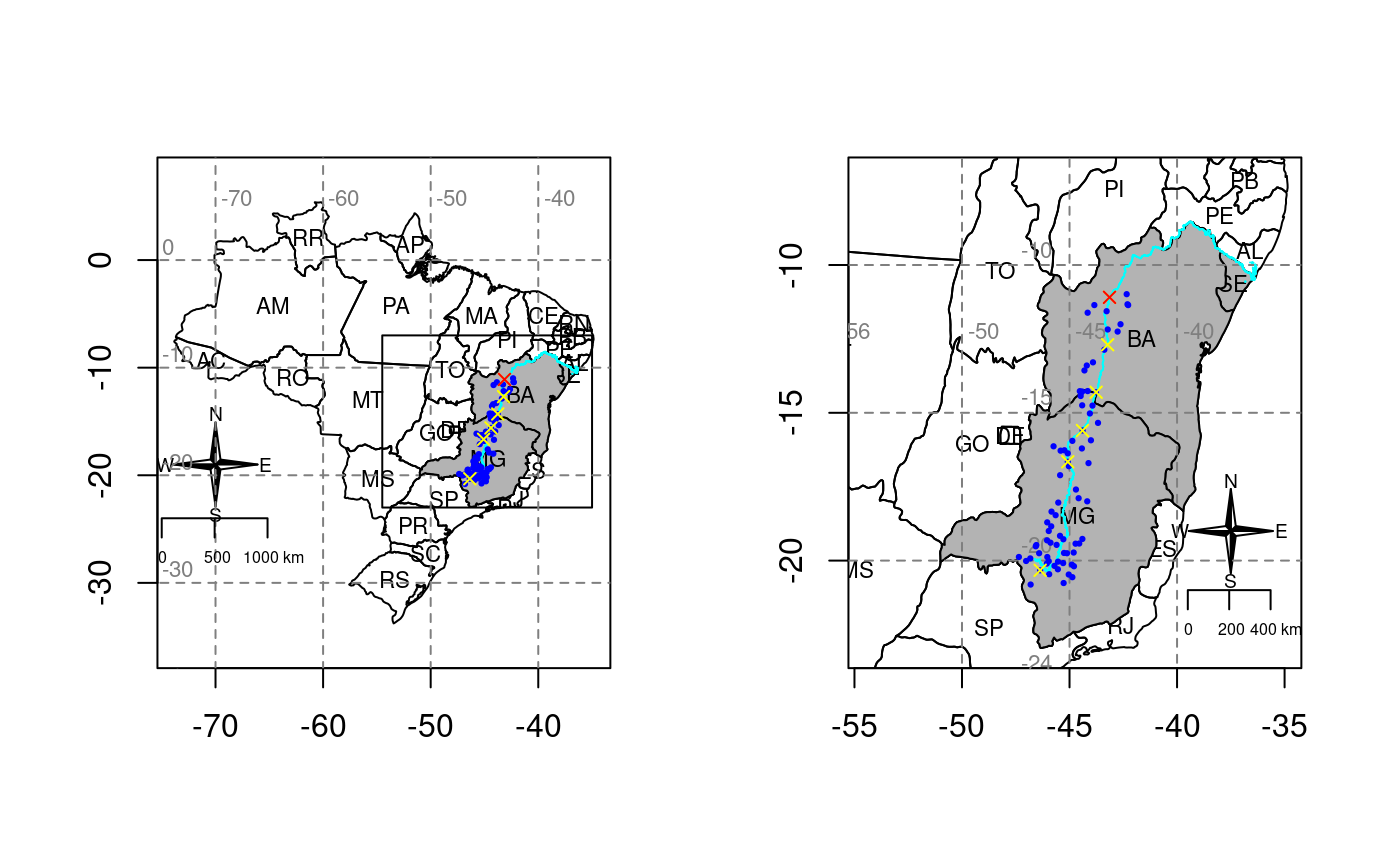
\includegraphics[width=0.9\linewidth]{figs/mapa} 

}

\caption{Mapa do percurso do rio São Francisco e a localização de suas estações pluviais e fluviais.}\label{fig:mapa}
\end{figure}

Sendo assim, foi selecionada aleatoriamente \(80\%\) dos dados para
construir o conjunto de treinamento e, portanto, \(20\%\) para teste.
Uma vez feita essa divisão do conjunto de dados em treino e teste, serão
ajustados diferentes modelo para estimar os valores da vazão segundo as
covariáveis e escolher aquele com maior poder preditivo

\hypertarget{modelo-de-regressuxe3o-linear-1}{%
\section{Modelo de regressão
linear}\label{modelo-de-regressuxe3o-linear-1}}

Inicialmente, foi ajustado um modelo de regressão linear para tentar
predizer a vazão com base em suas variáveis explicativas. Neste caso, o
modelo de regressão linear pode ser ajustado por meio da função
\textit{lm} e, com isso, obteve-se os resultados a seguir:

\begin{verbatim}
##        modelo MAE dentro MAE fora
## 1 Reg. Linear   157.8274 168.2205
\end{verbatim}

Uma outra forma de ver o desempenho do modelo é por meio da visualização
gráfica. Plotando os valores da variável \(y\) real contra os seus
respectivos valores preditos \(\widehat{y}\), espera-se um comportamento
próximo ao linear se os valores ajustados estiverem próximos aos
verdadeiros. Portanto, uma vez que as predições estão bem próximas da
linha vermelha que, nesta caso, representa o valor real da variável
\(y\), então pode-se afirmar que o modelo de regressão linear possui
precisão razoável para realizar as previsões para os dados da vazão.

\begin{figure}

{\centering 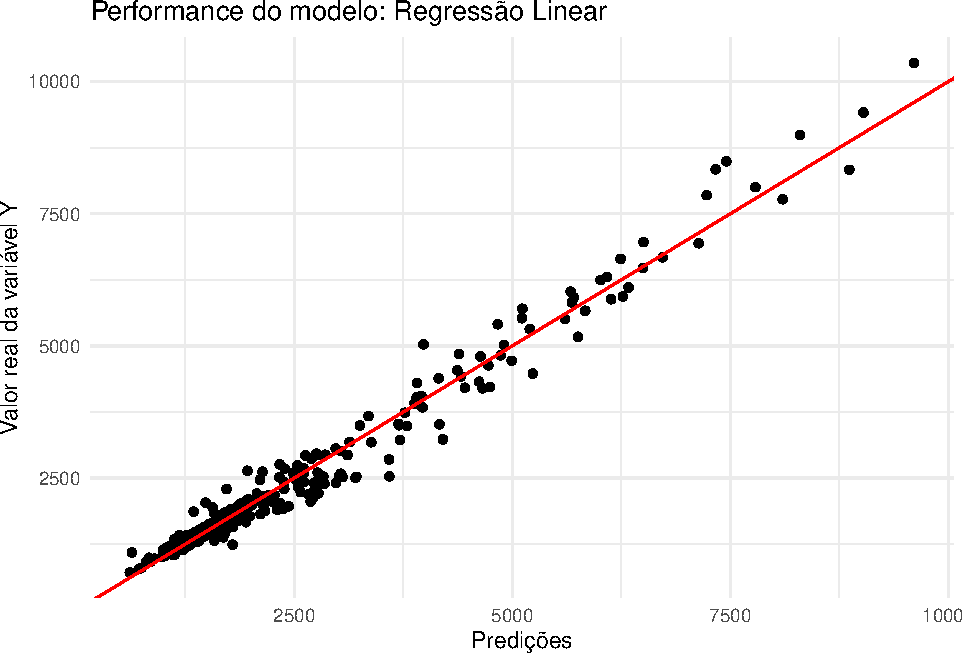
\includegraphics[width=0.6\linewidth]{figs/unnamed-chunk-6} 

}

\caption{Performance do modelo.}\label{fig:unnamed-chunk-6}
\end{figure}

\hypertarget{seleuxe7uxe3o-de-variuxe1veis-e-regularizauxe7uxe3o-1}{%
\section{Seleção de variáveis e
regularização}\label{seleuxe7uxe3o-de-variuxe1veis-e-regularizauxe7uxe3o-1}}

Considerando o método de seleção de variáveis \textit{Forward Stepwise}
(seleção progressiva), o tamanho do subconjunto selecionado com o
critério BIC foi igual a 15, de modo que as variáveis correspondentes
foram:

\begin{verbatim}
##  [1] "X40025000" "X42210000" "X44290002" "X45298000" "X46105000" "X46998000"
##  [7] "X1444004"  "X1645000"  "X1645005"  "X1744010"  "X1845013"  "X1945038" 
## [13] "X1946011"  "X2044006"  "X2047037"
\end{verbatim}

\noindent Note que estas variáveis são as que minimizam o critério BIC
(vejo o gráfico da figura \eqref{fig:BIC}) e, portanto, são
correspondentes ao melhor modelo dentre todos os possíveis utilizando um
subconjunto de variáveis que se dispõem.

\begin{figure}

{\centering 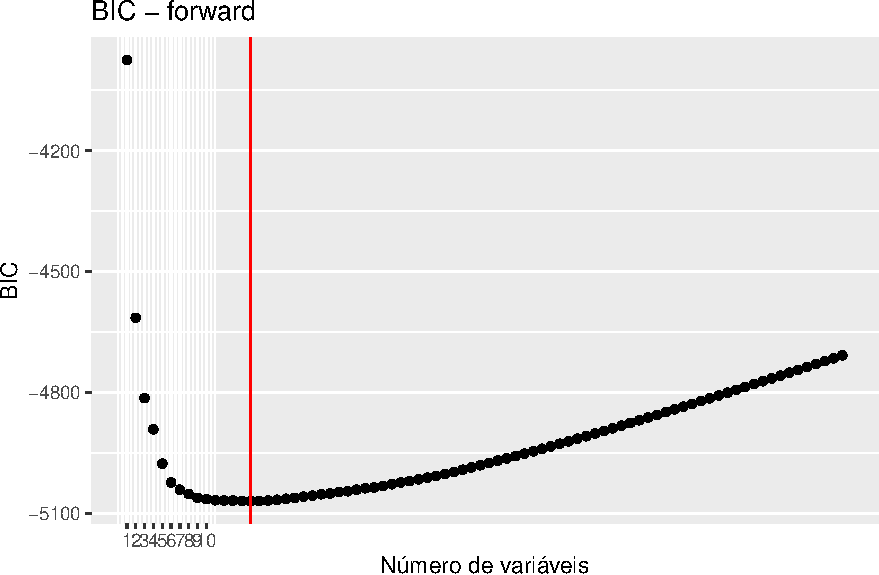
\includegraphics[width=0.6\linewidth]{figs/BIC} 

}

\caption{Seleção de modelo via Forward Stepwise.}\label{fig:BIC}
\end{figure}

\noindent Com isso, foi ajustado um modelo de regressão linear com as
variáveis selecionadas anteriormente o que resultou, respectivamente,
nos seguintes erros estimados dentro da amostra de treinamento e fora da
amostra no conjunto de validação.

\begin{verbatim}
##    modelo MAE dentro MAE fora
## 2 forward   162.6963 164.7212
\end{verbatim}

Considerando agora o método de seleção de variáveis
\textit{Backward Stepwise} (seleção regressiva), o tamanho do
subconjunto selecionado com o critério BIC foi igual a 14, de modo que
as variáveis correspondentes foram:

\begin{verbatim}
##  [1] "X40025000" "X42210000" "X44290002" "X45298000" "X46105000" "X46998000"
##  [7] "X1444004"  "X1645000"  "X1645005"  "X1744010"  "X1845013"  "X1945004" 
## [13] "X1946011"  "X2044006"
\end{verbatim}

\noindent Assim como na seleção progressiva, na seleção regressiva as
variáveis selecionadas são as que minimizam o critério BIC e
correspondem ao melhor modelo dentre todos os possíveis utilizando um
subconjunto de variáveis. Sendo assim, o modelo de regressão linear foi
ajustado com as variáveis selecionadas anteriormente o que resultou,
respectivamente, nos seguintes erros estimados.

\begin{verbatim}
##     modelo MAE dentro MAE fora
## 3 backward   163.5094 163.3929
\end{verbatim}

\noindent Neste caso, pode-se observar que o erro estimado fora da
amostra no conjunto de validação associado a este modelo selecionado
pelo método de \textit{Backward Stepwise} é melhor do que o obtido pelo
método \textit{Forward Stepwise} e pela regressão linear considerando
todas as variáveis. O desempenho considerando o conjunto de teste pode
ser visualizado graficamente.

\begin{figure}

{\centering 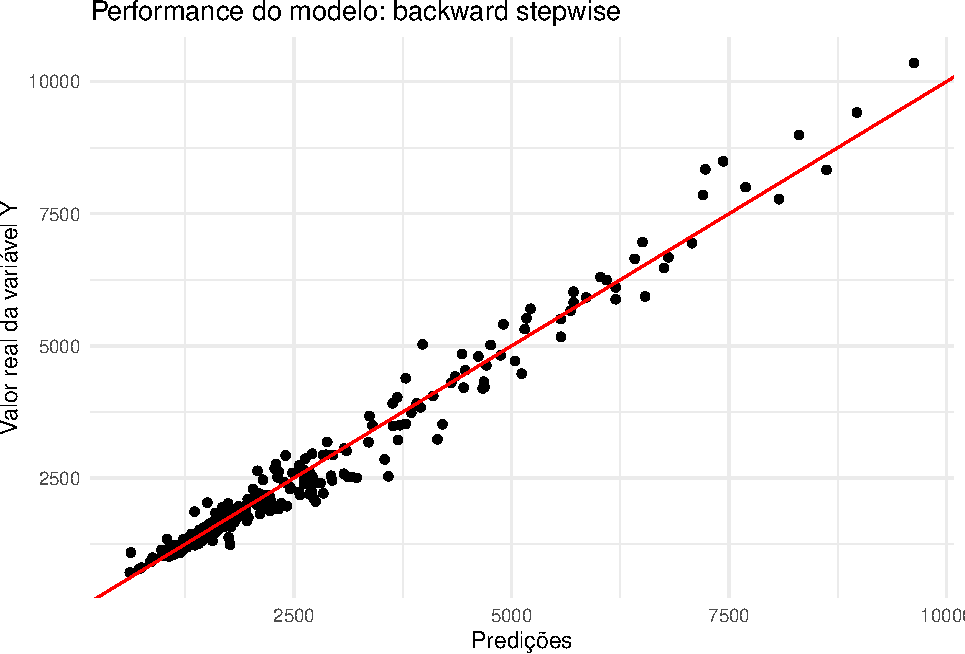
\includegraphics[width=0.6\linewidth]{figs/unnamed-chunk-9} 

}

\caption{Performance do modelo.}\label{fig:unnamed-chunk-9}
\end{figure}

Considerando o agora método de regressão linear com penalização LASSO,
por meio da validação cruzada, escolhemos o valor do hiperparâmetro de
penalização que minimiza o erro de validação cruzada (lambda.min), dado
por:

\begin{verbatim}
## [1] 6.792707
\end{verbatim}

\begin{figure}

{\centering 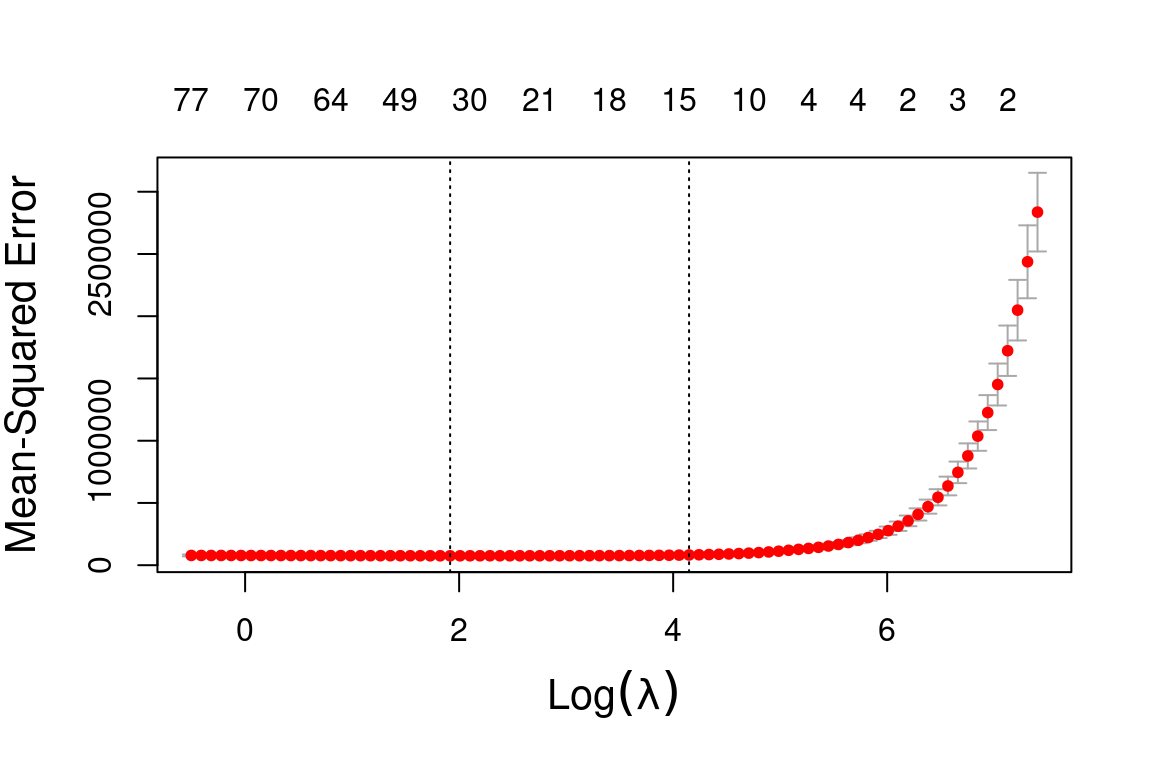
\includegraphics[width=0.6\linewidth]{figs/unnamed-chunk-10} 

}

\caption{Performance do modelo.}\label{fig:unnamed-chunk-10}
\end{figure}

\noindent Com isso, será ajustado um modelo de regressão linear com
penalização LASSO utilizando o valor de \(\lambda\) ótimo obtido
anteriormente o que resultou, respectivamente, nos seguintes erros
estimados dentro da amostra de treinamento e fora da amostra no conjunto
de validação.

\begin{verbatim}
##   modelo MAE dentro MAE fora
## 4  lasso   160.5908  158.688
\end{verbatim}

Neste caso, observa-se que o erro estimado fora da amostra no conjunto
de validação associado ao modelo de regressão linear com penalização
LASSO é melhor do que o obtido pela regressão linear sem regularização.
O desempenho considerando o conjunto de teste pode ser visualizado
graficamente.

\begin{figure}

{\centering 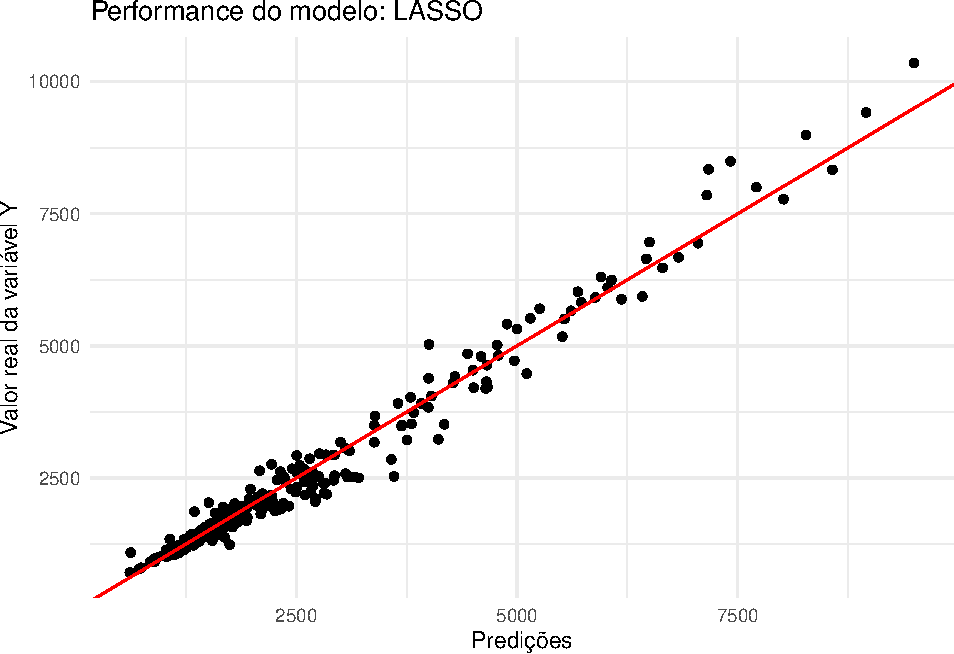
\includegraphics[width=0.6\linewidth]{figs/unnamed-chunk-11} 

}

\caption{Performance do modelo.}\label{fig:unnamed-chunk-11}
\end{figure}

De igual forma, considera-se agora o método de regressão linear, porém,
com penalização RIDGE. Aqui também foi necessário a validação cruzada
para escolher o valor do hiperparâmetro de penalização que minimiza o
erro de validação cruzada. Neste caso, o lambda selecionado foi de:

\begin{verbatim}
## [1] 164.3922
\end{verbatim}

\noindent Então, ajustando um modelo de regressão linear com penalização
RIDGE utilizando o \(\lambda\) ótimo obtido anteriormente, obtemos
respectivamente os seguintes erros estimados dentro da amostra de
treinamento e fora da amostra no conjunto de validação.

\begin{verbatim}
##   modelo MAE dentro MAE fora
## 5  ridge   157.4613 159.0079
\end{verbatim}

Observe então que embora o erro estimado dentro da amostra de
treinamento associado ao LASSO seja maior do que o obtido utilizando o
RIDGE, o erro estimado fora da amostra no conjunto de validação
associado do LASSO é menor. O desempenho considerando o conjunto de
teste pode ser visualizado graficamente.

\begin{figure}

{\centering 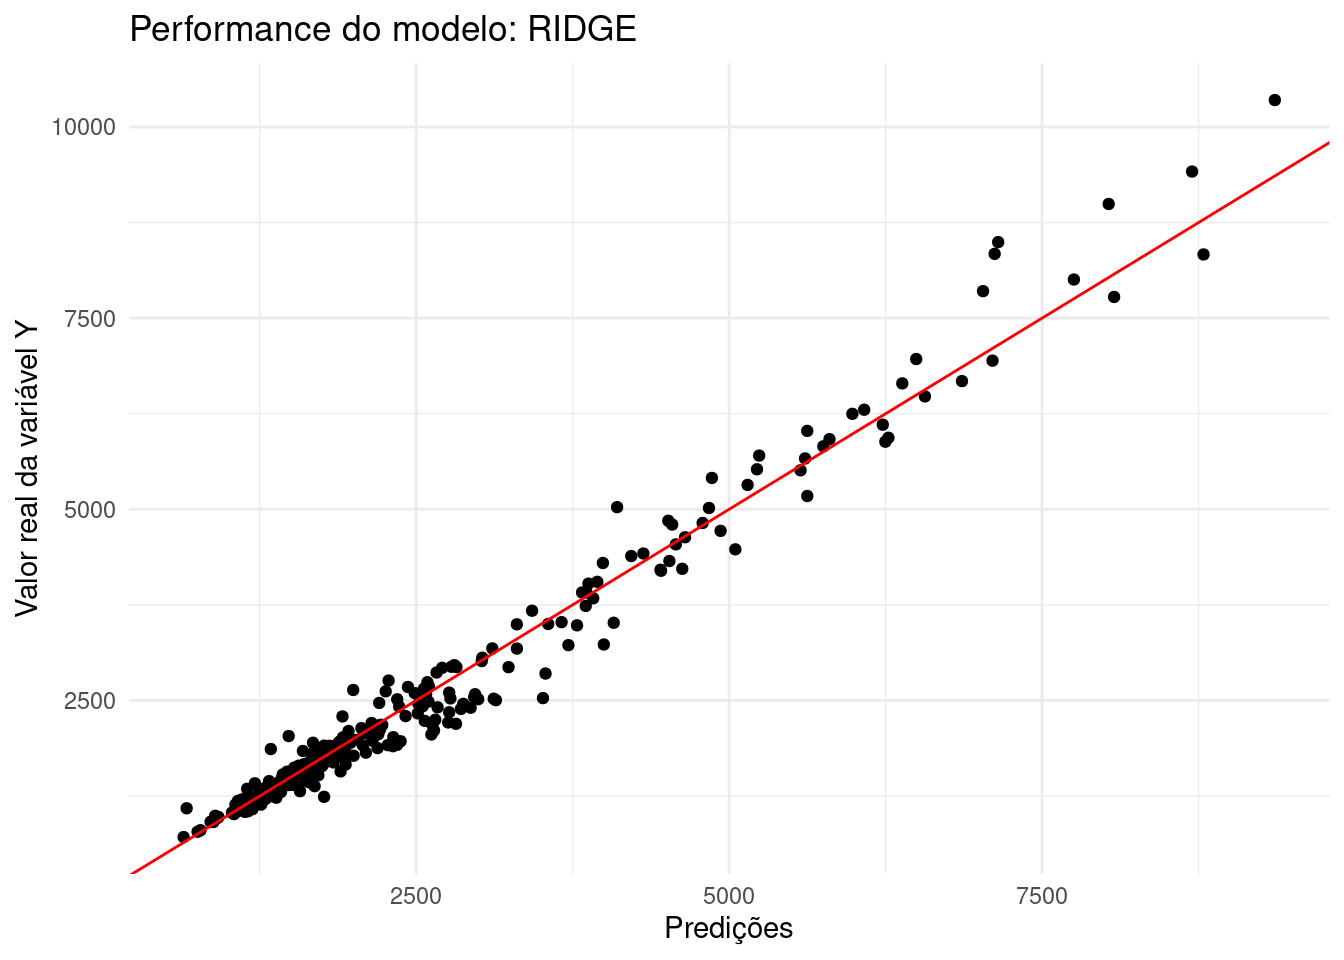
\includegraphics[width=0.6\linewidth]{figs/unnamed-chunk-12} 

}

\caption{Performance do modelo.}\label{fig:unnamed-chunk-12}
\end{figure}

Por fim, considerando agora o método de regressão ELASTIC NET, por meio
da validação cruzada, escolhemos o valor do hiperparâmetro de
penalização que minimiza o erro de validação cruzada, dado por:

\begin{verbatim}
## [1] 16.36368
\end{verbatim}

\noindent Desta forma, ajustando um modelo de regressão ELASTIC NET
utilizando o valor de \(\lambda\) ótimo obtido anteriormente, obtemos
respectivamente os seguintes erros estimados dentro da amostra de
treinamento e fora da amostra no conjunto de validação.

\begin{verbatim}
##        modelo MAE dentro MAE fora
## 6 elastic-net   160.5922 158.4374
\end{verbatim}

\noindent Neste caso, o erro estimado dentro da amostra de treinamento
associado ELASTIC NET é maior do que os demais métodos de regularização.
Contudo, o seu o erro estimado fora da amostra no conjunto de validação
é menor.

De forma geral, embora o ELASTIC NET tenha obtido desempenho melhor nas
predições no conjunto de validação, os métodos de regularização possuem
performance bem semelhantes entre si. Contudo, eles apresentam
resultados melhores do que os obtidos com a regressão linear sem
regularização.

\hypertarget{uxe1rvore-de-regressuxe3o}{%
\section{Árvore de regressão}\label{uxe1rvore-de-regressuxe3o}}

Em seguida, propomos agora um modelo de árvore de decisão no contexto de
regressão. Sendo assim, usando a função \textit{tree}, do pacote de
mesmo nome, ajustamos o modelo de árvore de regressão para explicar a
vazão dadas as demais variáveis consideradas.

\begin{verbatim}
## 
## Regression tree:
## tree(formula = Y ~ ., data = dados_tr)
## Variables actually used in tree construction:
## [1] "X45298000" "X44290002" "X46998000" "X46105000"
## Number of terminal nodes:  7 
## Residual mean deviance:  168100 = 229600000 / 1366 
## Distribution of residuals:
##     Min.  1st Qu.   Median     Mean  3rd Qu.     Max. 
## -2224.00  -213.60   -20.73     0.00   180.10  2374.00
\end{verbatim}

Observe que apenas quatro variáveis foram utilizadas na construção da
árvore, o que resultou em \(8\) nós terminais. Ou seja, tem-se uma
árvore \(T\) com \(8\) regiões. No contexto de árvore de regressão, o
desvio é simplesmente a soma dos erros quadrados da árvore. A seguir,
pode-se obsevar o plot da árvore.

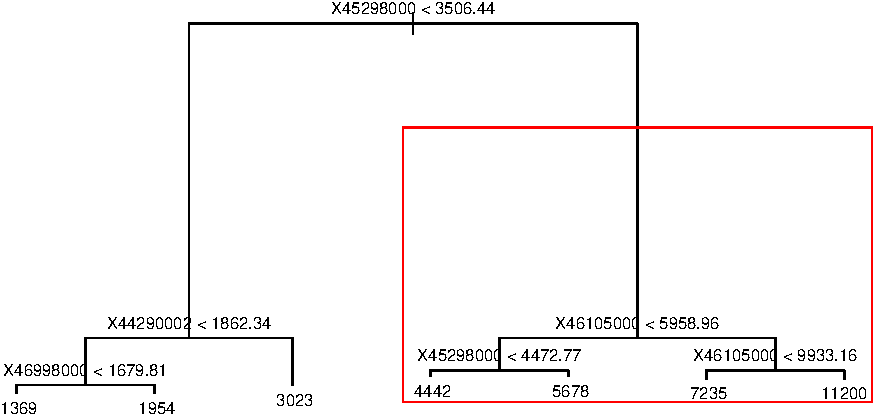
\includegraphics{figs/unnamed-chunk-13.pdf}

Para cada região, a predição é constante. Isto é, para todos os pontos
que caírem em uma determinada região, a predição para todos esses pontos
será a média de todos os pontos que caírem nessa região. Considere o
retângulo vermelho: observe que a região para qual todos os valores de
\(X45298000\) são tais que \(X45298000> 3506.44\), porém são também tais
que \(X46105000<5958.96\), bem como \(X46105000<4472.77\), então os
valores preditos da variável \(y\) será valor \(\hat{y}_{R_4} = 4442\).
Ou seja, para todos os pontos que caírem nessa região, o valor predito
de \(y\) será \(\hat{y}_{R_4} = 4442\), que corresponde a média de todos
os pontos que pertencem a essa região.Com isso, as predições da variável
\(y\) feita com base nessa árvore resultou nos seguintes erros absoluto
médio dentro e fora da amostra:

\begin{verbatim}
##   modelo MAE dentro MAE fora
## 7 arvore   282.7944 285.3219
\end{verbatim}

Uma vez que o modelo obtido pela árvore de regressão é um modelo
descontínuo, muitos pontos da amostra de teste vão ter o mesmo valor
predito. Então o gráfico de dispersão do valor real da variável resposta
\(y\) contra o seu valor predito \(\hat{y}\) será dado da seguinte
forma:

\begin{figure}

{\centering 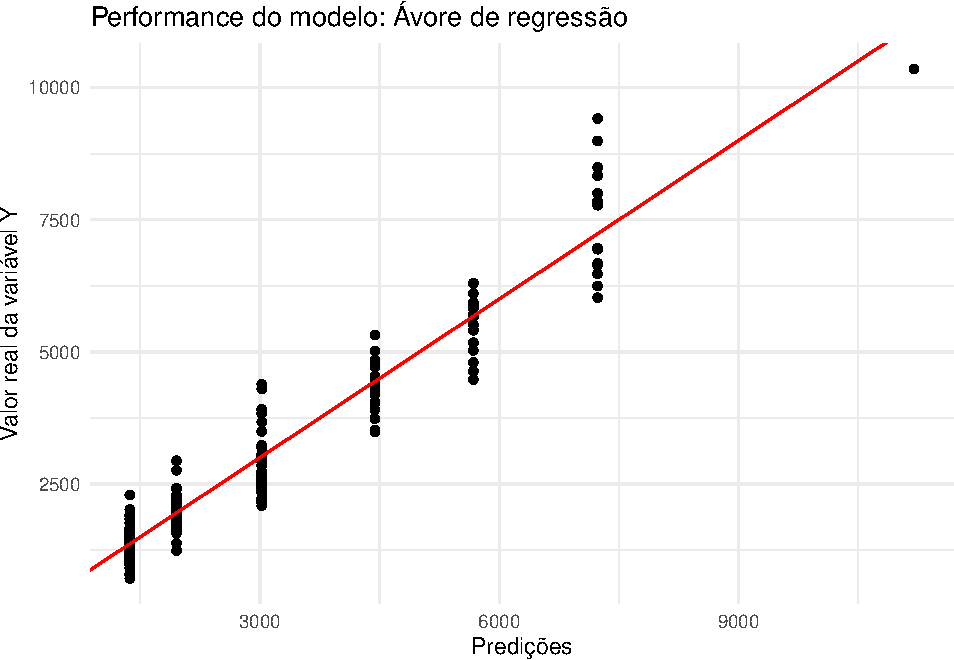
\includegraphics[width=0.6\linewidth]{figs/unnamed-chunk-15} 

}

\caption{Performance do modelo.}\label{fig:unnamed-chunk-15}
\end{figure}

\hypertarget{poda-da-uxe1rvore-1}{%
\subsection{Poda da árvore}\label{poda-da-uxe1rvore-1}}

Usando a validação cruzada para encontrar uma árvore considerando
árvores de diferentes tamanhos que foram podadas da árvore original,
obteve-se o seguinte gráfico com os tamanhos das árvores e as
respectivas raízes quadradas dos erros quadráticos médios.

\begin{figure}

{\centering 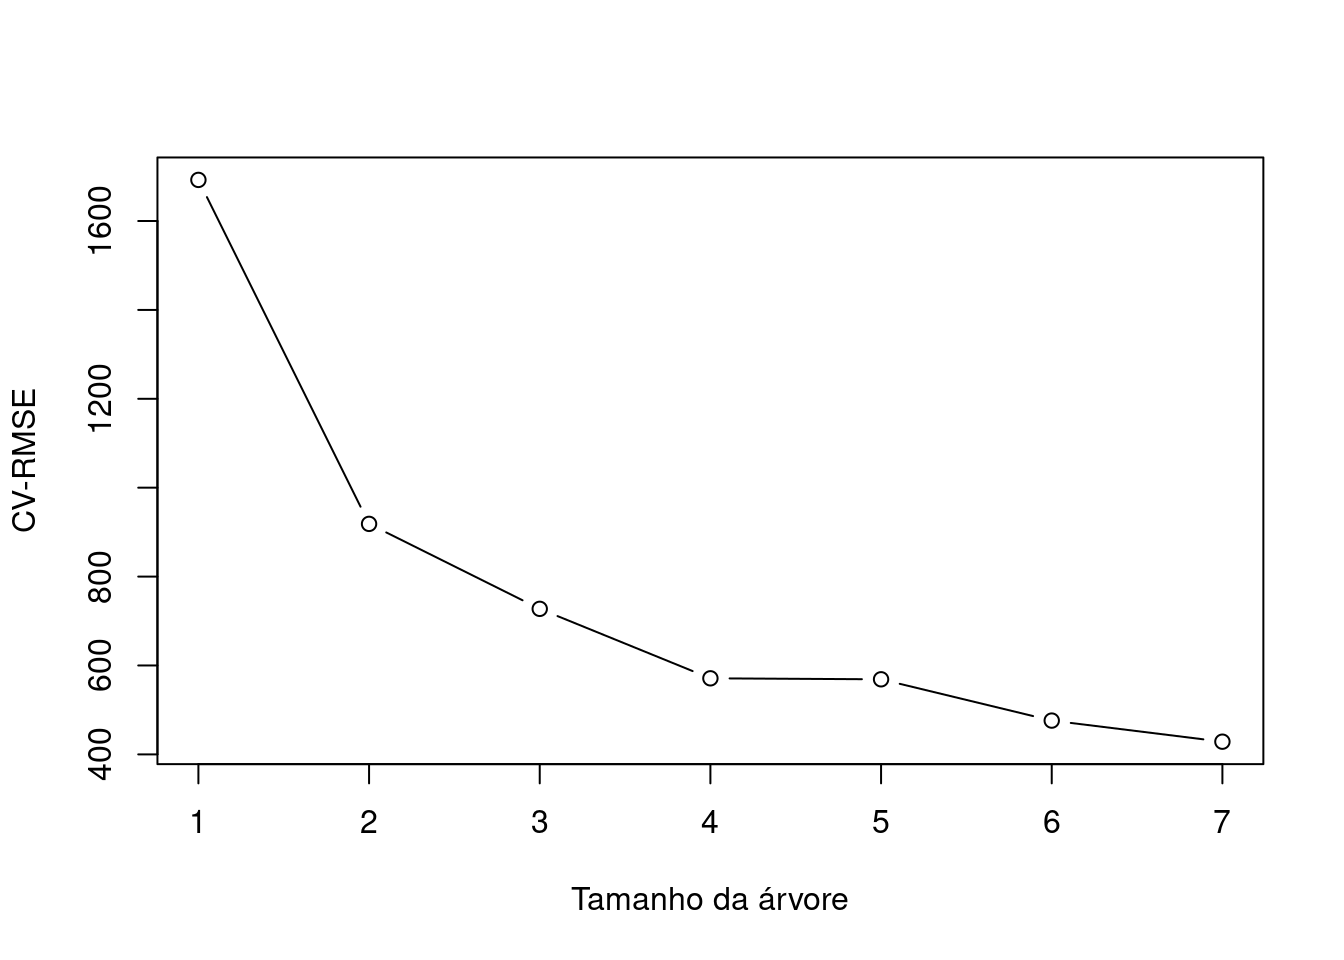
\includegraphics[width=0.8\linewidth]{figs/arvore_reg_pod_CV} 

}

\caption{Poda da árvore que gera o menor RMSE.}\label{fig:arvore_reg_pod_CV}
\end{figure}

Note que a árvore de 8 nós apresentou o MAE mais baixo obtido pela
validação cruzada e, portanto, não há melhora no modelo, tendo em vista
que o modelo anterior já tinha esse total de nós. Contudo, outra poda
será realizada para uma árvore de tamanho 4, pois parece que tem um
desempenho tão bom quanto, bem como também uma árvore podada é, como
esperado, menor e mais fácil de interpretar.

\begin{figure}
\centering
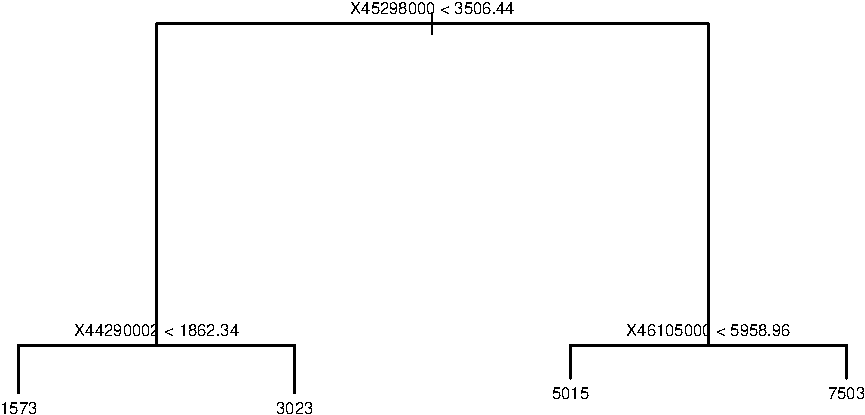
\includegraphics{figs/unnamed-chunk-16.pdf}
\caption{Gráfico da árvore podada.}
\end{figure}

Considerando essa árvore podada, as predições da variável \(y\) com base
na amostra de treinamento e amostra de teste resultou nos seguintes
erros dentro e fora da amostra:

\begin{verbatim}
##          modelo MAE dentro MAE fora
## 8 arvore podada   392.3105 397.3254
\end{verbatim}

\noindent Note que a árvore podada possui erro fora da amostra maior que
a árvore sem ser podada. Portanto, nesse caso, a árvore sem ser podada
tem precisão maior nas predições.

\hypertarget{muxe9todos-baseados-em-uxe1rvores-1}{%
\section{Métodos baseados em
árvores}\label{muxe9todos-baseados-em-uxe1rvores-1}}

\hypertarget{bagging-1}{%
\subsection{Bagging}\label{bagging-1}}

Com o objetivo de melhorar os resultados obtidos anteriormente, o método
bagging será proposto. Lembrando que o bagging é um caso particular do
floresta aleatória, e portanto todas as \(83\) variáveis preditoras são
considerados para cada divisão da árvore. Aqui, o modelo bagging foi
ajustado usando apropriadamente a função \textit{randomForest}. Neste
caso, por meio da amostra de teste e validação, foram obtemos os
seguintes erros estimados dentro e fora da amostra:

\begin{verbatim}
##    modelo MAE dentro MAE fora
## 9 bagging   52.73573 109.4501
\end{verbatim}

\noindent Pode-se observar então que há uma melhora expressiva
apresentado pelo baixo erro obtido fora da amostra, uma vez que as
predições estão bem próximas da linha vermelha que, nesta caso,
representa o valor real da variável \(Y\). Graficamente, tem-se que:

\begin{figure}

{\centering 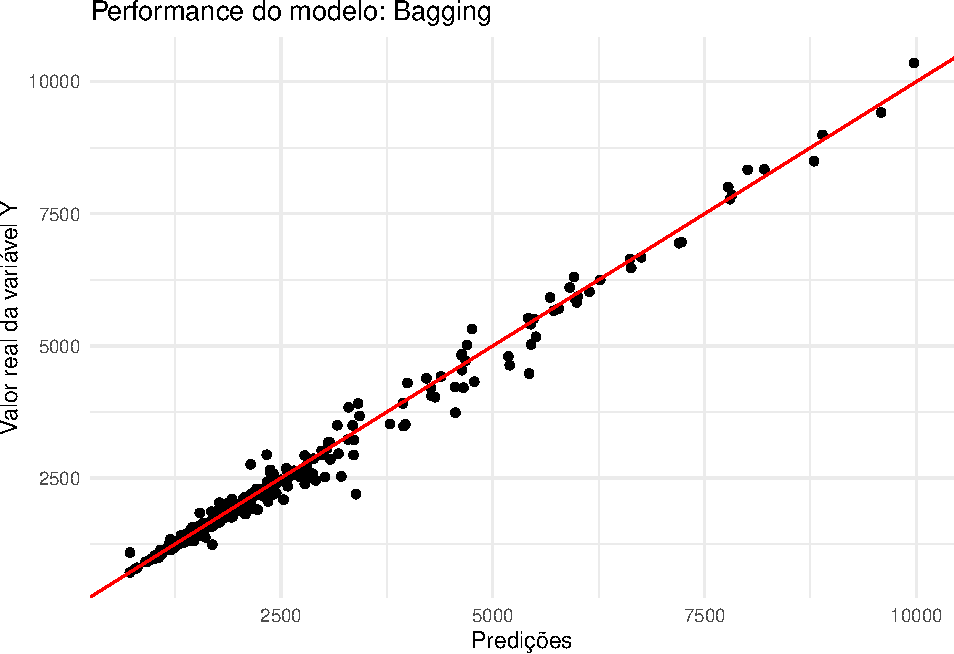
\includegraphics[width=0.6\linewidth]{figs/unnamed-chunk-17} 

}

\caption{Performance do modelo.}\label{fig:unnamed-chunk-17}
\end{figure}

\hypertarget{floresta-aleatuxf3ria}{%
\subsection{Floresta aleatória}\label{floresta-aleatuxf3ria}}

Neste caso, o modelo de floresta aleatória foi ajustado utilizando a
função \textit{randomForest} do pacote de mesmo nome, considerando como
\(27\) o número de variáveis aleatoriamente selecionadas como candidatas
em cada split. Portanto, obteve-se os seguintes erros estimados dentro
da amostra de treinamento e dentro da amostra no conjunto de teste:

\begin{verbatim}
## [1] 111.5726
\end{verbatim}

\begin{verbatim}
##    modelo MAE dentro MAE fora
## 10     rf   53.38865 111.5726
\end{verbatim}

\noindent Pode-se observar que os resultados são bastante similares aos
obtidos utilizado o bagging e que os dois reduzem bastante o erro obtido
com uma única árvore de regressão. O desempenho do modelo graficamente
pode ser observado a seguir:

\begin{figure}

{\centering 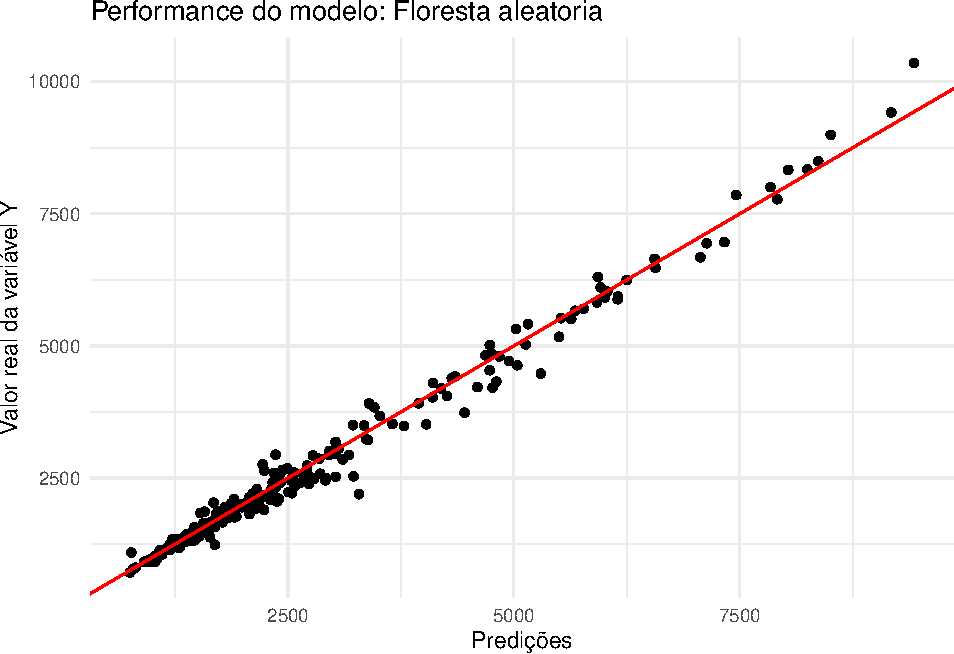
\includegraphics[width=0.6\linewidth]{figs/unnamed-chunk-18} 

}

\caption{Performance do modelo.}\label{fig:unnamed-chunk-18}
\end{figure}

\hypertarget{boosting-1}{%
\subsection{Boosting}\label{boosting-1}}

Agora será ajustado o boosting aos dados da vazão, por meio da função
\textit{gbm} do pacote de mesmo nome e, com isso, foram obtidos os
resultados a seguir:

\begin{verbatim}
##    modelo MAE dentro MAE fora
## 11    bst   136.5828 134.8408
\end{verbatim}

Sendo assim, é possível observar que o erro estimado dentro da amostra
de treinamento, bem como o erro estimado fora da amostra no conjunto de
validação associado ao boosting são maiores do que os obtidos usando o
bagging e o floresta aleatória, mas consideravelmente melhores do que
utilizando uma única árvore ou árvore podada de forma otimizada. O
desempenho considerando o conjunto de teste pode ser visualizado
graficamente.

\begin{figure}

{\centering 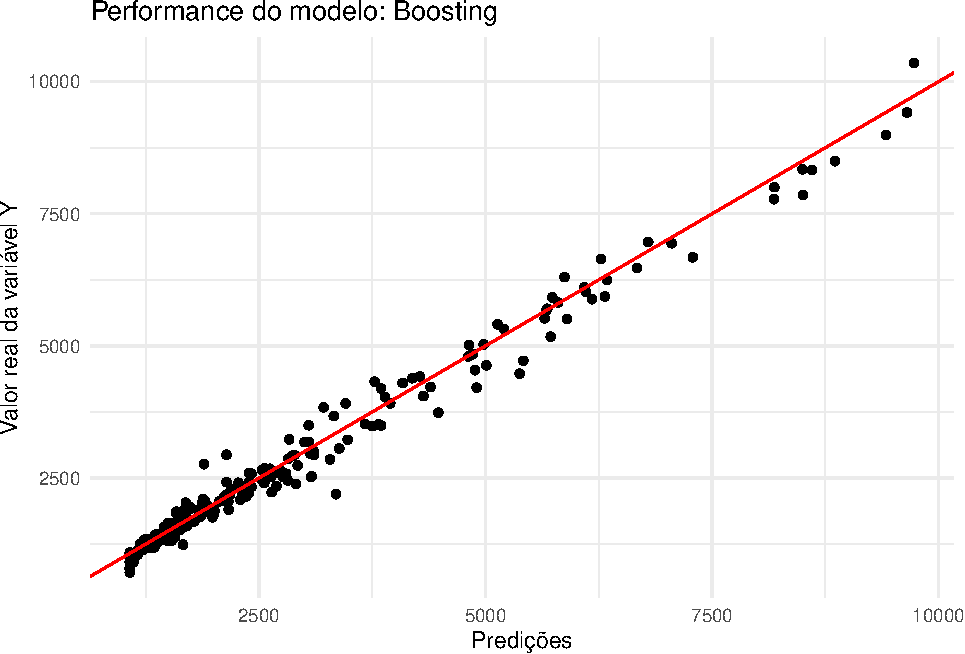
\includegraphics[width=0.6\linewidth]{figs/unnamed-chunk-19} 

}

\caption{Performance do modelo.}\label{fig:unnamed-chunk-19}
\end{figure}

\hypertarget{conclusuxe3o}{%
\section{Conclusão}\label{conclusuxe3o}}

Por fim, considerando o compartivo final, tem-se que:

\begin{verbatim}
##           modelo MAE dentro MAE fora
## 9        bagging   52.73573 109.4501
## 10            rf   53.38865 111.5726
## 11           bst  136.58280 134.8408
## 6    elastic-net  160.59216 158.4374
## 4          lasso  160.59082 158.6880
## 5          ridge  157.46132 159.0079
## 3       backward  163.50943 163.3929
## 2        forward  162.69634 164.7212
## 1    Reg. Linear  157.82736 168.2205
## 7         arvore  282.79436 285.3219
## 8  arvore podada  392.31045 397.3254
\end{verbatim}

\noindent Portanto, o modelo escolhido foi bagging, uma vez que o modelo
escolhido deve ser aquele com o menor erro na amostra de validação. Como
o menor erro de predição foi o obtido pelo bagging, concluí-se que este
é o melhor modelo para prever a vazão. Finalmente, considerando a
amostra inteira (treinamento mais teste) modelo escolhido foi treinado.
Posteriormente, foi utilizando os dados \textit{testesf}
disponibilizados para avaliar a performance do modelo preditivo.

Em conclusão, a aprendizagem estatística emerge como uma ferramenta
transformadora, capaz de extrair significado e valor de dados complexos.
Com isso, os modelos de aprendizado de máquina oferecem não apenas
eficiência operacional, mas também insights inovadores que impulsionam a
tomada de decisões informadas.





\newpage
\singlespacing 
\bibliography{master.bib}

\end{document}